In this chapter we review the thermodynamics of black holes as well as Hawking's information paradox. This paradox is solved by means of Quantum extremal surfaces (QES) \cite{almheiri2020entropy}.

\section{Black holes as thermal objects}

There were many hints indicating a relation between black holes and thermodynamics. For instance, the surface gravity $\kappa$ is constant over the event horizon of a stationary black hole. This motivates the zeroth law where, in thermodynamics, all parts of a system at thermodynamical equilibrium have equal temperature $T$. Also if one wants to study the behaviour of a QFT in a black hole spacetime, then the equilibrium of the system requires that the black hole has a temperature. This assigns a temperature to black holes and therefore they should be considered thermodynamical objects. And finally, we have an area theorem stating that the area of the event horizon is a non decreasing function of time. This suggests an analogy between black hole area $A$ and entropy $S$.

\subsection{First and second laws of thermodynamics}

In the 1970s, Bekenstein and others \cite{Bekenstein1972, PhysRevD.7.2333, PhysRevLett.25.1596} found equations that dictate black hole dynamics resembling those of thermodynamics,
\begin{equation}\label{1st law v1}
    \frac{\kappa}{8\pi G_N}\text{d}\left(\text{area}\right) = \text{d}M -\Omega\text{d}J + \phi\text{d}Q
\end{equation}
where $\kappa$ is the surface gravity, Area is that of its horizon, $M$ is its mass, $J$ the angular momentum, $\Omega$ is the rotational velocity of the horizon, $\phi$ the electric potential and $Q$ its charge. in this note, we are only interested in static neutral black holes where $J=0$ and $Q=0$.

If we postulate that the black hole entropy is proportional to the horizon area and has a temperature $\propto \kappa$, then (\ref{1st law v1}) looks exactly like the first law of thermodynamics
\begin{equation}\label{1st law v2}
    T\text{d}S_{\text{BH}} = \text{d}M -\Omega\text{d}J + \phi\text{d}Q.
\end{equation}
The reason why the entropy postulate makes sense, is that classically the area of the horizon is a non decreasing function of time. This resembles the second law of thermodynamics. The second law then reads\cite{Townsend:1997ku}: \begin{quote}
    If $T_{\mu\nu}$ satisfies the weak energy condition\footnote{The weak energy condition reads $v^\mu v^\nu T_{\mu\nu}\geq 0$ $\forall v$ non space-like. It is a condition that is used to constrain the solutions of Einstein field equations. It removes some solutions that are thought to be unphysical.}, and assuming that the cosmic censorship hypothesis\footnote{The cosmic censorship conjecture, proposed by Roger Penrose, states that there are no naked singularities, like a white hole, and therefore all singularities are hidden inside the event horizon. Up to this day, there is no rigorous proof of this conjecture. This is a major unsolved problem in classical G.R.} is true then the area of the future event horizon of an asymptotically flat spacetime is a non-decreasing function of time.
\end{quote}

This suggests that black holes are thermal objects. Indeed, Hawking discovered \cite{Hawking1975} that when coupled with quantum field theory, black holes have a temperature
\begin{equation}\label{Hawking temperature}
    T = \frac{\hbar \kappa}{2\pi}.
\end{equation}

If we consider the surrounding environment of a black hole, it could evaporate via Hawking radiations. Hawking radiation process can be interpreted as pair creation of entangled particles near the horizon, with one particle escaping to infinity and the other falling toward the singularity. Then the black hole slowly shrinks as its mass is carried away by the radiation. This would imply a decrease of the area in violation with the second law. We can solve this problem by assigning an entropy to the black hole as well as to the exterior. From (\ref{1st law v1}) and (\ref{Hawking temperature}), we find the total generalized entropy of a black hole to be
\begin{equation}\label{generalized entropy}
    S_{\text{gen}} = \frac{\text{Area}}{4\hbar G_N} + S_\text{outside},
\end{equation}
where $S_\text{outside}$ is the entropy of the QFT outside the horizon.

\section{Hawking information paradox}

Consider a black hole created from the collapse of a pure state. As time evolves, the black hole will emit thermal radiations. The origin of this thermal state is coming from entanglement as was discussed in the case of the thermofield double. As vacuum contains pairs of particles that are created and annihilated constantly, in the presence of a horizon things can be different. We can have one member of the entangled pair being absorbed by the horizon, while the other escapes it  and goes to infinity. This is the idea behind Hawking radiation \cite{Hawking1975}.

If we compute the entropy of radiations at early stages of evaporation, we will find it to be almost thermal as it is entangled with the quantum system and will start to increase as more Hawking quanta are emitted. However, as the black hole evaporates, its area becomes smaller and smaller, and therefore its thermal entropy (\ref{generalized entropy}) will decrease. As the black hole and the outside environment full of radiation, together, form a pure state, then by (\ref{Araki-Lieb}), $S_{\text{black hole}}=S_\text{rad}$. However, this fine-grained entropy cannot be bigger than the thermodynamic entropy (\ref{generalized entropy}), since it is not possible for the entropy of radiation to be entangled with a quantum system describing the black hole with fewer number of degrees of freedom (given by the thermodynamic entropy),
\begin{equation}
    S_{\text{black hole}}=S_\text{rad}\leq S_\text{Bekenstein-Hawking}.
\end{equation}

If the central dogma is to be true, then $S_\text{rad}$ should be expected to decrease once it becomes equal to $S_\text{Bekenstein-Hawking}$. The time at which this happens is called the Page time. The information paradox is summarized in figure \ref{Page curve}.

The Page time is achieved at an early stage compared to the Planck time $\sim 10^{-44}$s. So it should be possible to resolve this paradox in a semi-classical approximation.

\begin{figure}
    \centering
    \includegraphics[width=0.8\textwidth]{figures/page_island.png}
    \caption{Behaviour of radiation entropy during black hole evaporation. The increasing green curve is what was originally computed by Hawking. The decreasing orange curve is the thermodynamic entropy of the black hole. The Page curve in blue is the expected entropy in case we consider the central dogma hypothesis.}
    \label{Page curve}
\end{figure}

\section{Entropy of an evaporating black hole}

The central dogma considers the black hole and its surrounding region delimited by a cutoff surface to be equivalently described by a quantum system with large, but finite, degrees of freedom. The gravitational formula for the black hole von Neumann entropy is computed by minimizing (\ref{generalized entropy}) with respect to this cutoff surface
\begin{equation}\label{approx gravitational fine grained}
    S \sim \text{min}\left[\frac{\text{Area}}{4\hbar G_\text{N}} + S_\text{outside}\right].
\end{equation}

The actual formula is more than that. One equivalent definition is to take a Cauchy slice and find a minimal surface. Then choose the Cauchy slice that gives the maximum. The fine-grained entropy is then
\begin{equation}\label{gravitational fine grained}
    S = \min_X\left\{\text{ext}_X\left[\frac{\text{Area}\left(X\right)}{4\hbar G_\text{N}} + S_\text{semi-cl}\left(\Sigma_X\right)\right]\right\}.
\end{equation}
where $X$ is a codimension 2 surface called the quantum extremal surface (QES) and $\Sigma_X$ the slice on its left bounded by the cutoff surface as shown in fig. \ref{evaporation bh}.

When computing the fine grained entropy of the black hole using eq (\ref{gravitational fine grained}), we find two extremal quantum surfaces. The first case is the one with a vanishing surface. This contribution gives an increasing entropy as a function of time. The other extremal surface appears right after outgoing Hawking quanta escape the black hole. It lies close to the horizon. The generalized entropy now has a non vanishing area and the von Neumann entropy of the exterior quantum fields can be neglected. This entropy follows almost the shape of the thermodynamic entropy,
\begin{equation}
    S = \frac{\text{Area}_\text{hor}\left(t\right)}{4\hbar G_\text{N}}.
\end{equation}
Since (\ref{gravitational fine grained}) requires to take the minimum, we end up having an increasing entropy coming from the vanishing QES, and a decreasing entropy given by non vanishing QES. The overall shape of the curve follows the Page curve. The Page time is when the two extremal surfaces cross.

\begin{figure}
    \centering
    \begin{subfigure}[b]{0.3\textwidth}
        \centering
        \begin{tikzpicture}\label{evaporating bh}
            \draw (0,3) -- (0,-2.5)
            -- (5,2.5) -- (3,4.5)
            [sharp corners] -- (3,3);
            \draw [densely dotted] (0,0) -- (3,3);
           
            \fill[yellow, draw=black] (0,-2.5) .. controls (0.5,0.5) .. (0,3);
           
            \draw[densely dotted,color=blue] (0,-2.5) .. controls (3.5,3) .. (3,4.5);
           
            \draw[color=green] (0.5,1) parabola (2.5,1.5);
           
            \filldraw[green] (0.5,1) circle (2pt) node[anchor=west] {~~~~~~~~~~~$\Sigma_X$};
            \node[above right=.5pt of {(.5,1)}, outer sep=2pt, color=green] {$X$};
           \draw[decorate,decoration=zigzag] (0,3)
           -- (3,3);
        \end{tikzpicture}
        \caption{}
        \label{evaporation bh}
    \end{subfigure}
    \hfill
    \begin{subfigure}[b]{0.3\textwidth}
        \centering
        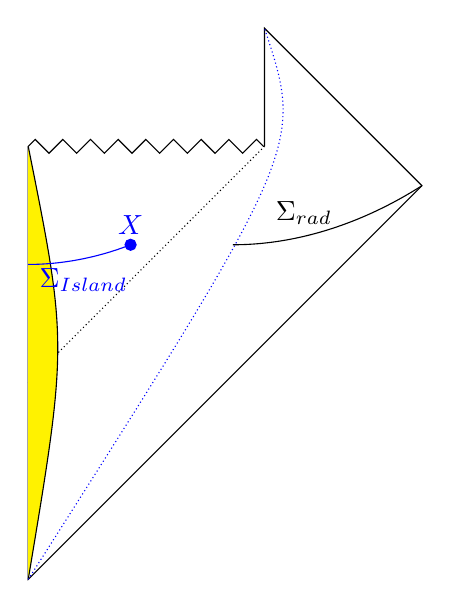
\begin{tikzpicture}
            \draw (0,3) -- (0,-2.5)
            -- (5,2.5) -- (3,4.5)
            [sharp corners] -- (3,3);
            \draw [densely dotted] (0,0) -- (3,3);
           
            \fill[yellow, draw=black] (0,-2.5) .. controls (0.5,0.5) .. (0,3);
           
            \draw[densely dotted,color=blue] (0,-2.5) .. controls (3.5,3) .. (3,4.5);
            \draw (2.6,1.75) parabola (5,2.5);
            \draw[color=blue] (0,1.5) parabola (1.3,1.75);
            
            \filldraw[blue] (1.3,1.75) circle (2pt) node[anchor=south] {$X$};
            \draw[blue] node at (.7,1.3){$\Sigma_\text{Island}$};
           \draw[decorate,decoration=zigzag] (0,3)
           -- (3,3);
           %\draw[->]   (3.5,1.8) -- + (1,-1);
           %\draw[blue] node at (4.5,.6){$\Sigma_\text{rad}$};
           \draw node at (3.5,2.15){$\Sigma_\text{rad}$};
        \end{tikzpicture}
        \caption{}
        \label{evaporation rad}
    \end{subfigure}
    \caption{Penrose diagram of an evaporating black hole. The black hole is considered to be formed from the collapse of a pure state. (a) The quantum extremal surface for computing the fine grained entropy of the black hole. (b) The quantum extremal surface for computing the fine grained entropy of radiation. In this case we have a possible contribution coming from inside the horizon (the Island) which results in the decrease of the entropy.}
    \label{island radiation}
\end{figure}


This does not solve the Hawking information paradox yet, since it involves the entropy of radiations. However, we can use the same formula (\ref{gravitational fine grained}) to compute radiation entropy. There is no reason why $\Sigma_X$ cannot be disconnected. Indeed that is exactly the case for Hawking radiations. Computations through gravitational path integral suggest to include the interior for the black hole as well \cite{Marolf_2021}. This interior region behind the horizon that is included in the computation of radiation entropy is called an island. The fine grained entropy becomes
\begin{equation}\label{rad fine grained}
    S = \text{min}_X\left\{\text{ext}_X\left[\frac{\text{Area}\left(X\right)}{4\hbar G_N} + S_\text{semi-cl}\left(\Sigma_\text{Rad}\cup\Sigma_\text{Island}\right)\right]\right\}
\end{equation}
where the area is the boundary of the Island, figure \ref{island radiation}.

The straightforward possibility is the case with no island. In this case radiation entropy just increases as computed by Hawking. After some time, of order $r_s\log S_{BH}$, a non-vanishing island that extremises (\ref{rad fine grained}) appears. Since the von Neumann entropy includes the region inside the black hole, the entropy decreases over time. This is due to the interior Hawking quanta purifying the exterior modes\footnote{A very good analogy was given at the end of section 8 of \cite{almheiri2020entropy}.}. The minimum of the two extremums follows exactly the Page curve.
